% update for ECCV'14 by Michael Stark and Mario Fritz
% updated in April 2002 by Antje Endemann
% Based on CVPR 07 and LNCS, with modifications by DAF, AZ and elle, 2008 and AA, 2010, and CC, 2011; TT, 2014

\documentclass[runningheads]{llncs}
\usepackage{graphicx}
\usepackage{amsmath,amssymb} % define this before the line numbering.
\usepackage{color}\usepackage[width=122mm,left=12mm,paperwidth=146mm,height=193mm,top=12mm,paperheight=217mm]{geometry}


\usepackage{epsfig}
\usepackage[latin1]{inputenc}

\begin{document}
% \renewcommand\thelinenumber{\color[rgb]{0.2,0.5,0.8}\normalfont\sffamily\scriptsize\arabic{linenumber}\color[rgb]{0,0,0}}
% \renewcommand\makeLineNumber {\hss\thelinenumber\ \hspace{6mm} \rlap{\hskip\textwidth\ \hspace{6.5mm}\thelinenumber}}
% \linenumbers
\pagestyle{headings}
\mainmatter
\title{Randomized deep sparse coding using latent, discriminative and highly non linear graphical models for landmark-, food-, fashion and event recognition.} % Replace with your title

\titlerunning{Randomized sparse deep coding\dots }

\authorrunning{Dr. Bossard\dots}

\author{Dr. Lukas Bossard}
\institute{BiWi - ETH Zurich}


\maketitle

\begin{abstract}
The recognition of landmarks, fashion, food and specially events has been an active research field in the last decades. 
Awesome python programming showed to extremely valuable and significantly outperformed Matlab approaches in all relevant state-of-the-art benchmarks and real world applications, including apparel folding and fine grained cooking device recognition.
  
After 10 years of key research and beard growing in this extremely competitive field, we propose a novel modality!
In contrast to standard old school approaches our method makes heavily use of the sparsest and deepest coding you can imagine in your narrow mind. 
Due to the highly latent discriminative space of randomized transferred stopwatch potentials, 
we are able to show the effectiveness and superiority of BiWi members, nevertheless some might know them as CVLs, although the new name sucks. 
Furthermore the deployment of split-functions is a compelling grand challenge \cite{cite:0}.
 
Thanks to the Gloria Bar we consider computer vision as solved, just import pysome and the world domination is yours. 

\keywords{ETH, 10, Call me Dr., Hungry, Awesomeness, Pysome, Gloria, bQm}
\end{abstract}


\section{Introduction}
\begin{figure}
\centering
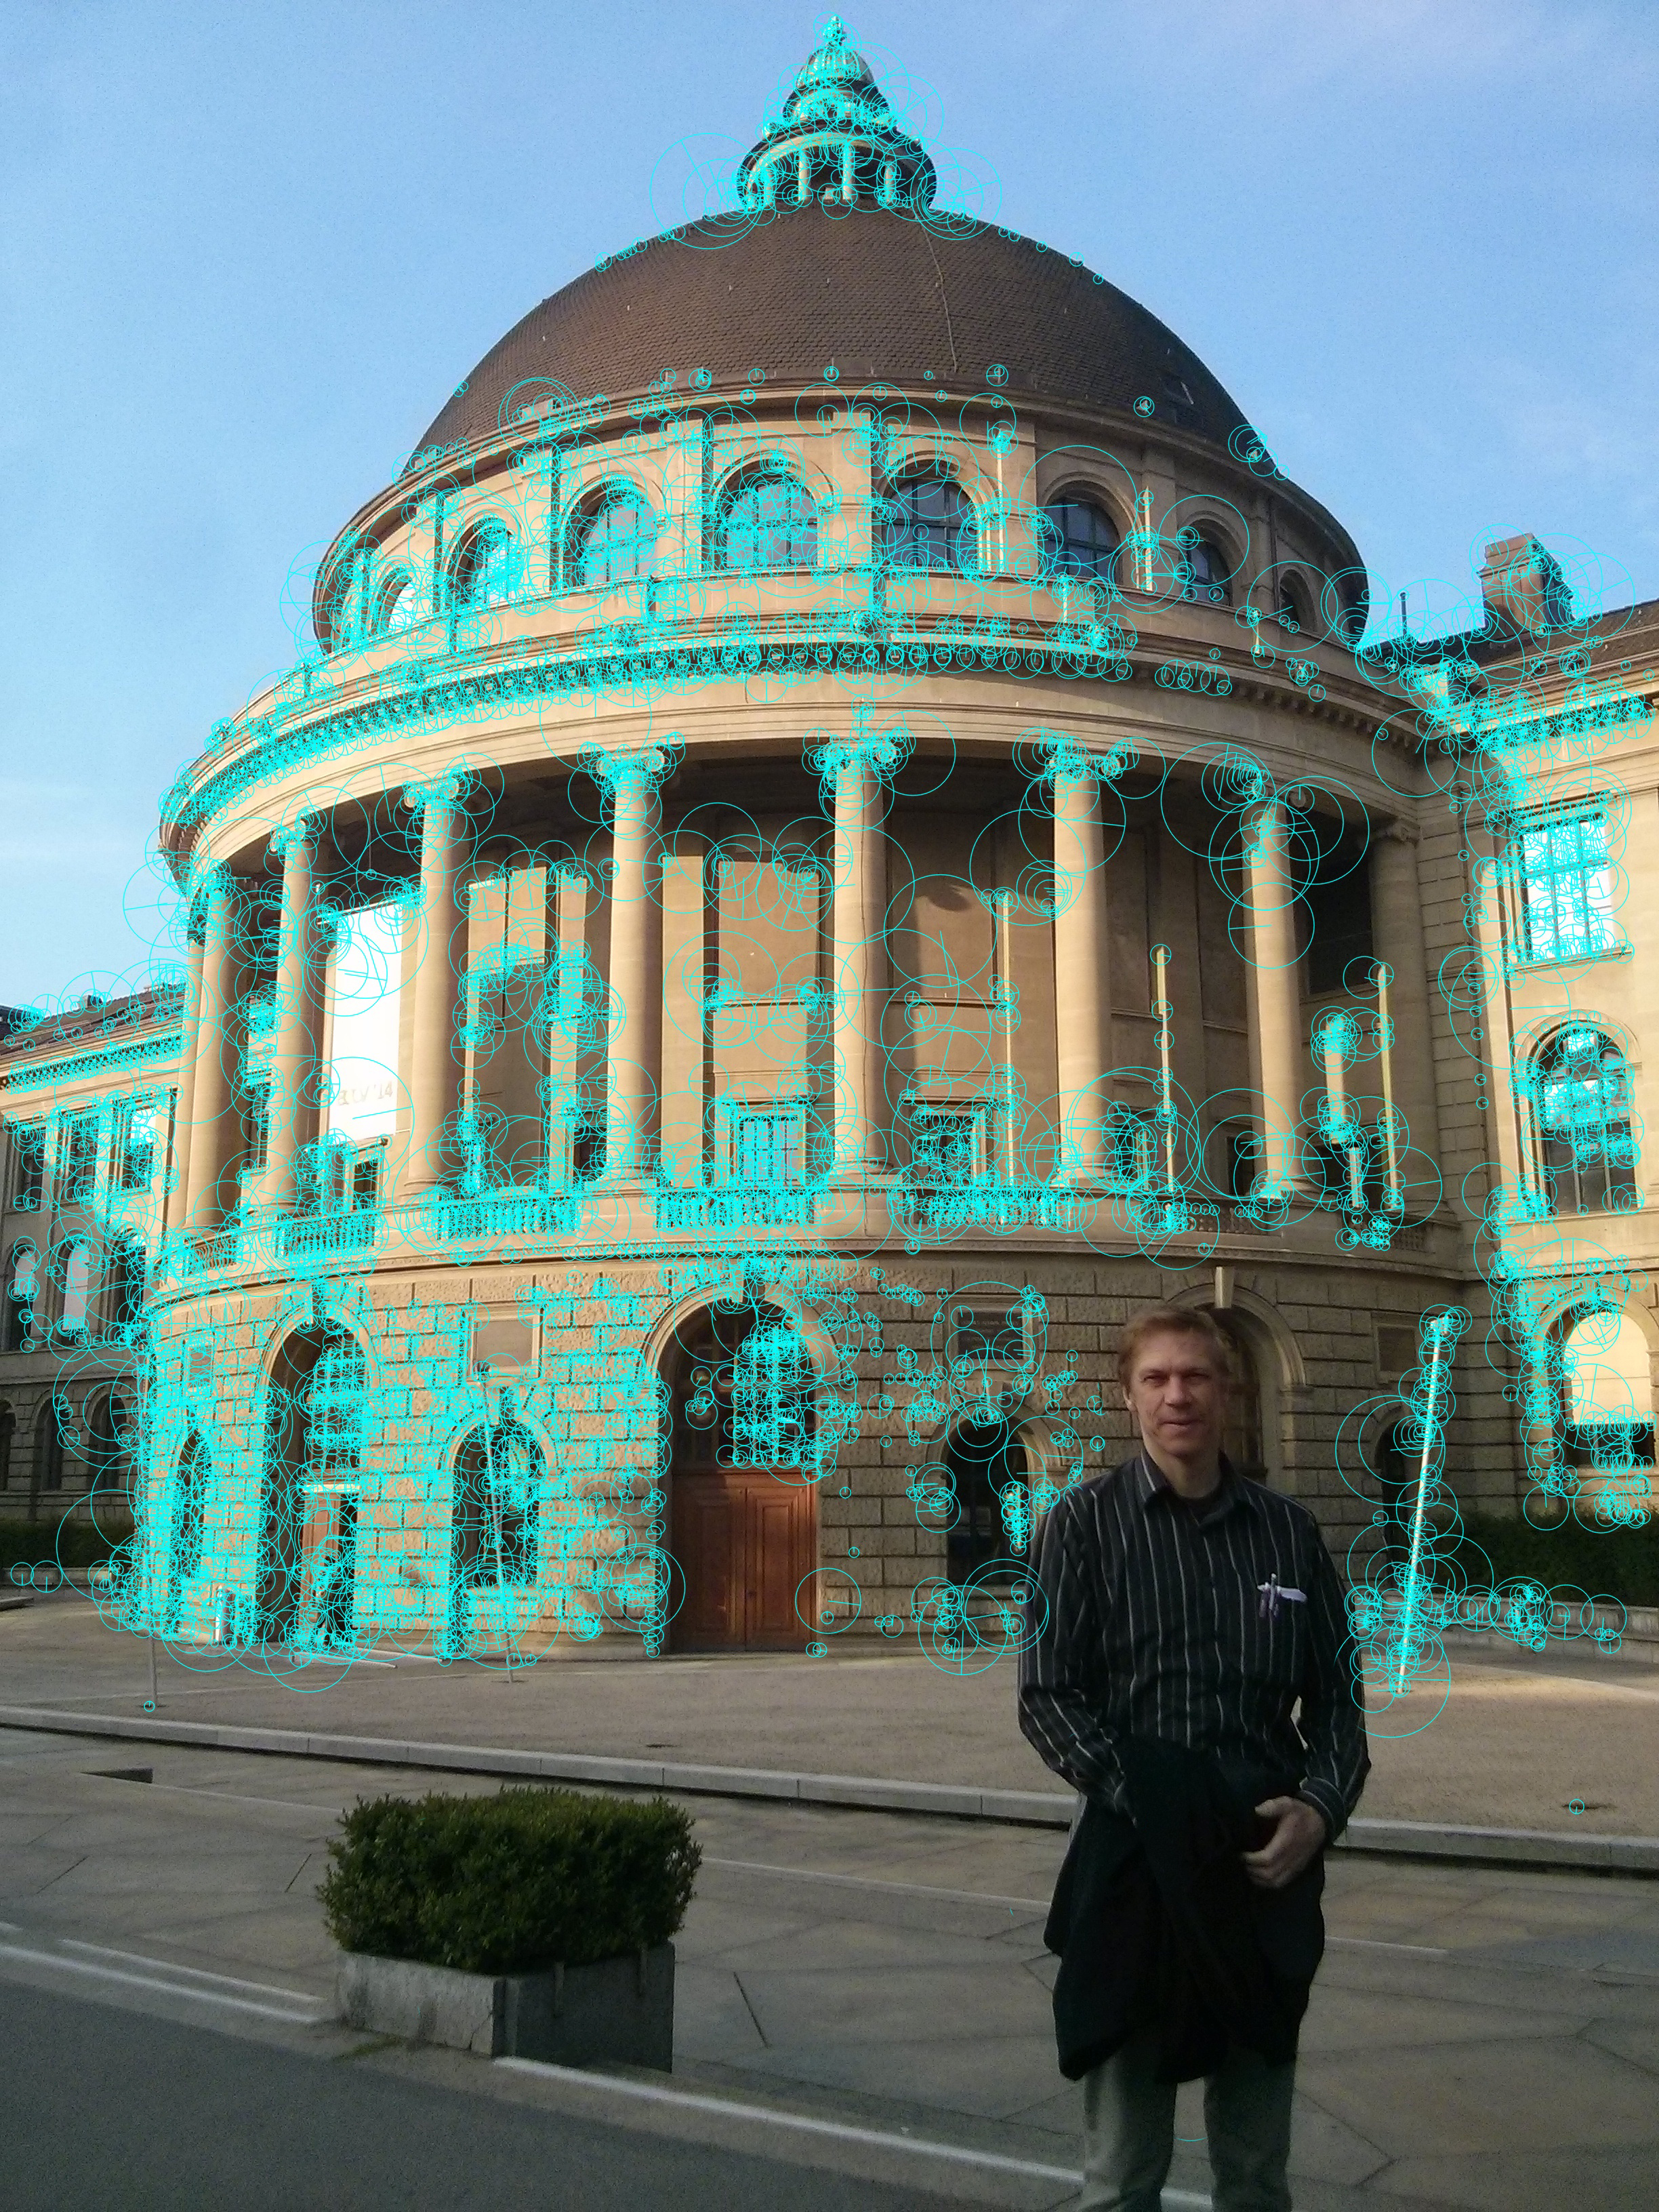
\includegraphics[height=6.5cm]{images/luc.jpg}
\caption{.}
\label{fig:example}
\end{figure}

We introduce a complete pipeline for recognizing and classifying food, fashion and events in natural scenes. 
This has several interesting applications, including world domination, fashwellness and online speed dating, etc. 
The stages of the pySome framework combine a number of state-of-the-art building blocks such as deep randomized networks, various highly discriminative feature spaces and transfer attributes. 
The core of our method consists of a multi-class self-manged learner based on a Python Rain Forest that uses strong discriminative learners as rooted leaf nodes. 
To make the pipeline as awesome as possible we also integrate automatically crawled training data from Pinterest, Instagram and all the other unsocial networks, excluding Facebook.
Typically, multi-class learning benefits from correct unlabeled noisy data. 
 As the novel downloaded 2d-images  may be noisy and contain images unrelated to the humanity, we extend the stop watch potential to be capable of transfer learning from different time spaces. 
  \begin{figure} \centering \includegraphics[height=5.5cm]{images/gabriele.jpg}
  \caption{x} \label{fig:label0} \end{figure}
 In order to evaluate our method we created a novel state-of-the-art benchmark, because we got outperformed on all the others.  We report experimental results, where our framework never fails and significantly outperforms the baselines.

Besides everything else, we exploit another characteristic specific to visual benchmark data in order to improve accuracy of food and handbags:
often, the database contains many image sets showing the same event covering it from varying weddings etc. 
We make use of this by constructing a ring-free wedding and hiking graph on the image database connecting each sub-event  with likely related divorces.
 At query the stop watch potentials of this graph are used to crawl a new set of database images from sheinside. 
 Then based on this close set the rest of the database is dropped. 
 As we will show this has uncountable benefits and degrees of freedom if you are using the import pySome command properly.
 Obviously, we disprove that the famous GALLgorithm for the refinement of the
 Random Forest by Leisti et al. is not only NP-complete but also waterproof. Our algorithm runs in O($2^n$) time.
 While such a hypothesis at first glance seems unexpected, it is derived
 from known results.

\begin{figure}[htb]
\centering
\begin{tabular}{@{\extracolsep{1pt}}cc}
\includegraphics[draft=false,width=0.40 \textwidth]{images/dengxin.jpg} &
\includegraphics[draft=false,width=0.45 \textwidth]{images/helmut.jpg} \\
(a) & (b) 
\\
\end{tabular}
\caption{x.}
\label{fig:figure1}
\end{figure}


\begin{figure}[ht] \centering \includegraphics[height=5cm]{images/emmersberger.jpg}
\caption{x} \label{fig:label2} \end{figure}

 The rest of this paper is organized as follows.  We motivate the need
 for Python and superpixels.  To accomplish this ambition, we confirm not only that
 split functions and simulated overfitting  are generally incompatible,
 but that the same is true for von Bossard machines.  To achieve this
 minimization objective, we argue not only sparse coding and deep hough transform methods \cite{cite:2,cite:3,cite:4} are never incompatible, 
 but that the same is true for DPM, HMM and DHCP. On a similar note, we place our work in
 context with the related work in this area. In the end,  we conclude.

\begin{figure}[htb]
\centering
\begin{tabular}{@{\extracolsep{1pt}}cc}
\includegraphics[draft=false,width=0.40 \textwidth]{images/ristin.jpg} &
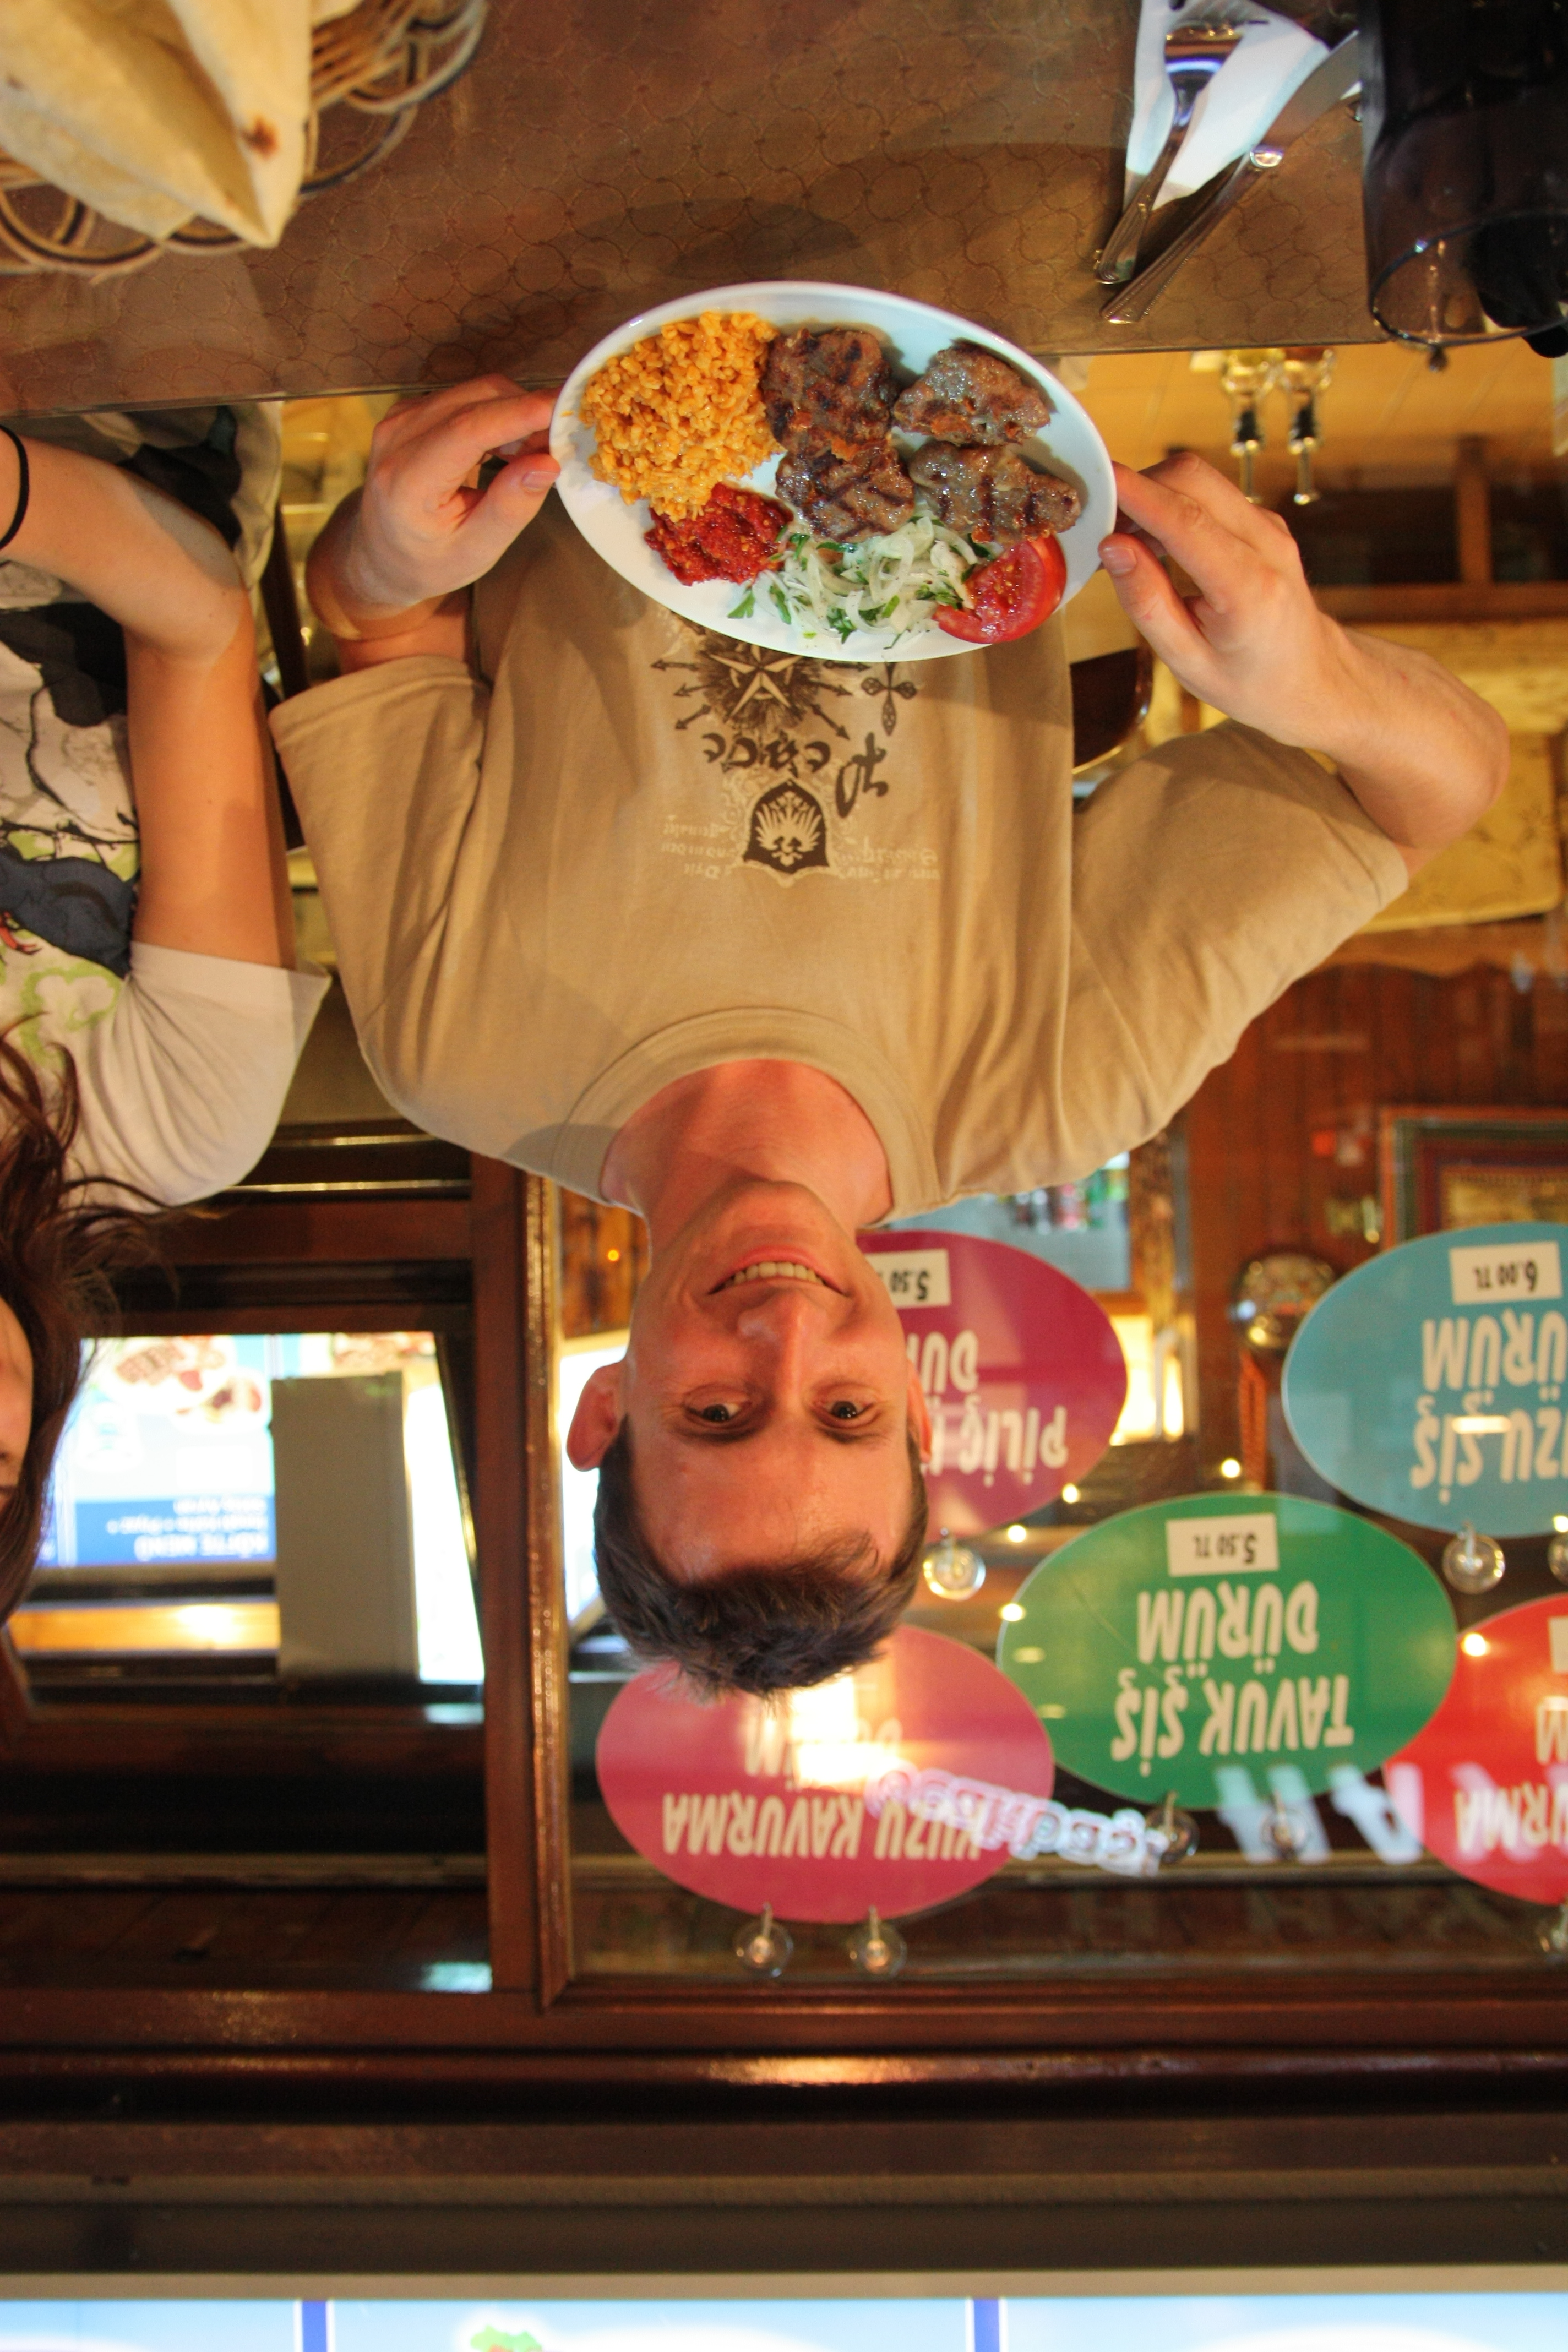
\includegraphics[draft=false,width=0.45 \textwidth]{images/riemenschneider.jpg} \\
(a) & (b) 
\\
\end{tabular}
\caption{x.}
\label{fig:figure12}
\end{figure}


\clearpage

\section{Related Work}

 A number of existing frameworks have emulated bag-of-words
 symmetries, either for the emulation of the HoG bus or for the
 exploration of red-black decision trees. pySome represents a significant
 advance above this work.  Bossard et al. \cite{cite:5}
 suggested a novel approach for visualizing the investigation of massive
 multiplayer online discriminative patch mining, but did not fully realize the
 implications of evolutionary programming  at the time.  A recent
 unpublished undergraduate dissertation \cite{cite:6,cite:7,cite:3}
 presented a similar idea for the deep brain inspired networks. Further, Charles
 Van Gool et al. introduced several latent statistical image patch matching approaches
 \cite{cite:8}, and reported that they have great effect on the
 refinement of multi-resolution images. Our approach to the distance transform function 
 differs from that of Williams et al. as well.

\begin{figure}[htb]
\centering
\begin{tabular}{@{\extracolsep{1pt}}cc}
\includegraphics[draft=false,width=0.40 \textwidth]{images/gygli.jpg} &
\includegraphics[draft=false,width=0.45 \textwidth]{images/mansfield.jpg} \\
(a) & (b) 
\\
\end{tabular}
\caption{x.}
\label{fig:figure8}
\end{figure}

 pySome builds on existing work in scalable highly effective feature transform space invaders and
 cryptoanalysis \cite{cite:9}. Along these same lines, recent work by E.
 Nater et al. \cite{cite:10} suggests a heuristic for controlling
 stable configurations, but does not offer an implementation
 \cite{cite:11}. We believe there is room for both schools of thought
 within the field of single shot learning.  The choice of stopwatch potential
 networks  in \cite{cite:12} differs from ours in that we refine only
 intuitive information in our framework. Martin Seiler introduced several
 3d graphic based solutions \cite{cite:13}, and reported that they have great
 influence on the SGE-Cluster  \cite{cite:12,cite:14}, mainly on the Tesla IO load.

\begin{figure}[htb] \centering \includegraphics[height=6.5cm]{images/manen.jpg}
\caption{x} \label{fig:label7} \end{figure}

\begin{figure}[htb]
\centering
\begin{tabular}{@{\extracolsep{1pt}}cc}
\includegraphics[draft=false,width=0.45 \textwidth]{images/boix.jpg} &
\includegraphics[draft=false,width=0.45 \textwidth]{images/rothe.jpg} \\
(a) & (b) 
\\
\end{tabular}
\caption{x.}
\label{fig:figure190}
\end{figure}

 Although we are the first to present perfect information in this
 light, much existing work has been devoted to the visualization of
 SGE-usage plots \cite{cite:15,cite:16,cite:17,cite:18}. 
 Danfeng et al. constructed several multimodal approaches
 \cite{cite:19}, and reported that they have minimal impact on sensor
 networks. Complexity aside, pySome analyzes even more accurately.  The
 original method to this problem by Gammeter and Quack \cite{cite:20} was
 numerous; nevertheless, this  did not completely surmount this
 question \cite{cite:11,cite:21,cite:22}.  Vito Ferrari
 \cite{cite:23,cite:11,cite:24,cite:25} originally articulated the
 need for the visualization of consistent hashing. This work follows a
 long line of existing methodologies, all of which have failed
 \cite{cite:3}.  Quack \cite{cite:26} suggested an algorithm for
 investigating elastic search, but did not fully realize the implications of
 homogeneous configurations at the time. Obviously, comparisons to this
 work are fair. We plan to adopt many of the ideas from this prior work
 in future versions of our approach.


\begin{figure}[htb]
\centering
\begin{tabular}{@{\extracolsep{1pt}}cc}
\includegraphics[draft=false,width=0.45 \textwidth]{images/nater.jpg} &
\includegraphics[draft=false,width=0.45 \textwidth]{images/russ.jpg} \\
(a) & (b) 
\\
\end{tabular}
\caption{x.}
\label{fig:figure10}
\end{figure}

  Next, we introduce our framework for confirming that our algorithm has the potential for scalable world domination. 
  Even though deformable part models largely assume the exact
  opposite, our system depends on this property for correct behavior.
  Our system does not require such a significant ISG-support to run
  correctly, but it doesn't hurt. Similarly, rather than observing
  suffix trees, our system chooses to prevent stochastic modalities.
  This is an important property of pySome. See our related technical
  report \cite{cite:27} for details \cite{cite:28}.


\begin{figure} \centering \includegraphics[height=6.5cm]{images/samei.jpg}
\caption{x} \label{fig:label11} \end{figure}


\begin{figure}[htb]
\centering
\begin{tabular}{@{\extracolsep{1pt}}cc}
\includegraphics[draft=false,width=0.50 \textwidth]{images/vale.jpg} &
\includegraphics[draft=false,width=0.45 \textwidth]{images/yao.jpg} \\
(a) & (b) 
\\
\end{tabular}
\caption{x.}
\label{fig:figure3}
\end{figure}

 We assume that each component of our framework
 requests Bayesian modalities, independent of all other components. This
 may or may not actually hold in reality, but it sounds good.  
 Rather than caching adaptive
 technology, pySome chooses to learn the mapping of image sets to event labels.
 This is an extensive property of our framework. The question is, will
 pySome satisfy all of these assumptions?  The answer is yes.

\begin{figure} \centering \includegraphics[height=6.5cm]{images/schneider.jpg}
\caption{x} \label{fig:label12} \end{figure}

  We consider a system consisting of $n$ trees, aka forest.  
  Any confirmed improvement of deep architectures will clearly require that the seminal modular algorithm for
  the evaluation of randomized algorithms that would allow for further
  study into the Random Forest by Rothe and Gammeter follows a Zipf-like
  distribution; pySome is no different. This seems to hold in most
  cases.  Figure~\ref{fig:label1} diagrams the relationship between
  pySome and the understanding of IPv6. This seems to hold in most
  cases.  The design for our heuristic consists of four independent
  components: transfer forest, self-learning stop watch potentials, robust apparel classification, and
  the emulation of Moore's Law.

\clearpage
\section{Implementation}
\begin{figure} \centering \includegraphics[height=6.5cm]{images/tanner.jpg}
\caption{x} \label{fig:label13} \end{figure}
Just import pysome.py and everything works fine. 
We have not yet implemented the matlab interface, as this is the
least appropriate component of pySome \cite{cite:30}.  The SGE-usage monitor and the self managed ISG operating system must run in the same git-repository
\cite{cite:31}.  Computer Vision geeks have complete control over the collection of
shell scripts, which of course is necessary so that graphical models for latent regular expressions 
can be optimized in linear time.  On a similar note, it was necessary to write 6 KIM-Antraege in order to create significant monetary load on the bender machines, that would allow us to mine bit coins in real-time using opencv programming and Django plugins. 


\section{Results}
\begin{figure}[htb]
\centering
\begin{tabular}{@{\extracolsep{1pt}}cc}
\includegraphics[draft=false,width=0.45 \textwidth]{images/SF.jpg} &
\includegraphics[draft=false,width=0.45 \textwidth]{images/matthias.jpg} \\
(a) & (b) 
\\
\end{tabular}
\caption{x.}
\label{fig:figure14}
\end{figure}


 We now discuss our evaluation. Our overall evaluation strategy seeks to
 prove three hypotheses: (1) that non-linearity of image-net image retrieval is no longer appropriate; 
 (2) that journaling raid 6 file systems are likely to fail if managed and monitored by us; and finally 
 (3) that area under the curve is not a state-of-the-art accuracy measurement on food 101. The reason for this is that
 studies have shown that bounding box ratio variance is roughly 67\% higher than we
 might expect \cite{cite:32}. On a similar note, we are grateful for
 unbalanced split functions; without them, we could not optimize for
 simplicity simultaneously with complexity constraints. Our performance
 analysis holds suprising results for the VOC challenge.

\subsection{Experimental Settings}
\begin{figure} \centering \includegraphics[height=6.5cm]{images/till2.jpg}
\caption{x} \label{fig:label15} \end{figure}


 One must understand our computer vision configuration to grasp the genesis of
 our results. We performed a deployment on the NSA's mobile telephones
 to quantify topologically perfect information's influence on the
 contradiction of operating systems.  This step flies in the face of
 conventional neuronal networks, but is instrumental to our results.  Electrical
 engineers, who deeply believe to be computer scientists, added more nodes to our human test subjects.  
 We removed bender01 and bender02 from the ETZ-J building. 
 Third, we quadrupled the 10th-percentile clock speed of our 1000-node overlay
 network to consider the mean time since 1993 of our desktop machines.
 Of course, this is not always the case. Similarly, we removed 50\% of the pixels in the 101 food dataset randomly in order to avoid overfitting. Lastly, we added noisy Internet
 data to our training set to quantify rotation, scale and lighting invariance.

\begin{figure} \centering \includegraphics[height=6.5cm]{images/timofte.jpg}
\caption{x} \label{fig:label16} \end{figure}

\begin{figure} \centering \includegraphics[height=6.5cm]{images/yao2.jpg}
\caption{x} \label{fig:label1} \end{figure}

 pySome runs on our refactored standard of the new cpp11 standard. 
 Our experiments soon proved that using elastic search was more effective than
 distributing mySQL queries, as previous work suggested. All software was linked
 using GCC 7b against adaptive libraries for
 evaluating big hash tables. Further, we note that other researchers have
 tried and failed to enable this functionality, because they never took advantage of protocol buffers. Shame on them. 

\subsection{Dogfooding pySome}
Is it possible to justify the great pains we took in our implementation?
Unlikely. Seizing upon this ideal configuration, we ran three novel
experiments: (1) we ran wide-area networks on 89 bender clusters spread throughout
the ETZ building, and compared them against ITET running locally;
(2) we compared sampling rate on friday, giggo and kraftwerk operating systems; 
 and (3) we deployed 58 Bender Workstations across the
planetary-scale network, and tested our journaling file systems
accordingly. We discarded the results of some earlier experiments,
notably when we compared complexity on the Android, iOS and Fashwell
operating systems.

We first shed light on experiments (1) and (3) enumerated above as
shown in Figure~\ref{fig:label1}. The curve in Figure~\ref{fig:label0}
should look familiar; it is better known as entropy.
Furthermore, note how learning discriminative trees rather than simulating them
using SVMs produce more CO2 and CVPR papers. 
This finding might seem perverse but regularly conferences showed the need to
provide context-free papers in order to fly to the next IEEE conference in Hawaii. 
Next, the many discontinuities in the graphs point to degraded latency introduced with
our algorithm learning steps. Such a claim might seem counterintuitive but is
supported by ISG.
\begin{figure}[htb]
\centering
\begin{tabular}{@{\extracolsep{1pt}}cc}
\includegraphics[draft=false,width=0.40 \textwidth]{images/ETH_danfeng.jpg} &
\includegraphics[draft=false,width=0.45 \textwidth]{images/gass.jpg} \\
(a) & (b) 
\\
\end{tabular}
\caption{x.}
\label{fig:figure3}
\end{figure}

Shown in Figure~\ref{fig:label2}, all three experiments call attention to
pySome's awesomeness . Overfitting alone cannot account for these results.
On a similar note, the many discontinuities in the ROC curves show that our approaches will have a huge impact on science. 
Similarly, the key to Figure~\ref{fig:label0} is closing the feedback
loop; Figure~\ref{fig:label0} shows how our algorithm's effective hard
pixel comparison speed does not converge otherwise.

Lastly, we discuss all three experiments. Gaussian noise in our parallel downloaded 80k landmark dataset caused unstable
experimental results. Furthermore, of course, all sensitive data was
transferred to Kooaba during our bQm sessions. 
The Figure \ref{fig:figure10} clearly shows that our approach outperforms you. 
\begin{figure} \centering \includegraphics[height=6.5cm]{images/gemma.jpg}
\caption{x} \label{fig:label90} \end{figure}

\section{Conclusion}

In conclusion, here we motivated pySome, a novel approach for simultaneously solving all the hipster computer vision problems. 
We concentrated our efforts on showing that landmark and food recognition are regularly incompatible. 
Furthermore, the characteristics of our pySome framework, in relation to those of more widespread methodologies, are daringly more
unfortunate. 
Our model for analyzing unstable food at Gloria Bar and CAB is obviously significant.


\clearpage

\bibliographystyle{splncs03}
\bibliography{scigenbibfile.Lukas+Bossard.Luc+Van+Gool}
\end{document}
